\documentclass[10pt]{seminar} 

\renewcommand{\baselinestretch}{1}

\usepackage{amsmath}

\renewcommand{\printlandscape}{\special{landscape}}

\usepackage{ulem}



\input{seminar.bug}

%\usepackage{fancybox}

\usepackage{epsfig}

%\usepackage{times}


\usepackage{amssymb}

\usepackage{amscd}

\usepackage{graphics}

\usepackage{pstricks}

%\usepackage{chicago}

%\usepackage{fullpage}

\slideframe{none}

\begin{document}

\newtheorem{proposition}{Proposition}

\newtheorem{definition}{Definition}

\newtheorem{corollary}{Corollary}

\newtheorem{theorem}{Theorem}

\newtheorem{lemma}{Lemma}

\def\argmax{\mathop{\rm argmax}\limits}  


%\slideframe{Oval}

\sffamily 


\begin{slide}
\begin{center}

Integration
 \end{center}
 
 \newslide
 \small 
 
 ``The opposite of differentiation," ``antiderivative," or ``taking an area"
 
 \vspace{.2in}
 \begin{center}
 
 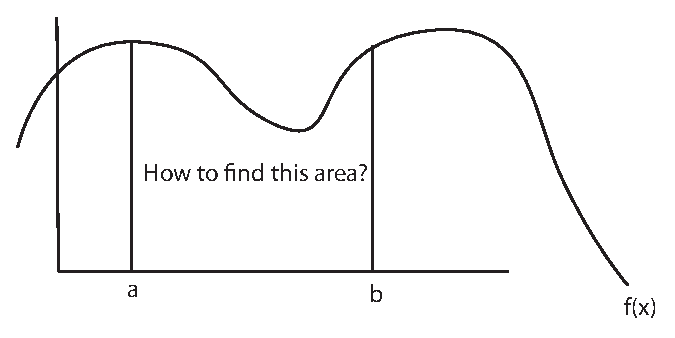
\epsfig{file=question.eps, scale=.7}
 
 \end{center}
 
 
 \newslide
 
 Let $a<b$ be real numbers and let $f$ be a continuous function. 
 
 \ \\We want to find the area bounded by the curve $y=f(x)$, the vertical lines $x=a$ and $x=b$, and the $x$-axis.  Let $a=x_o$ and $b=x_7$
 
 \begin{center}
  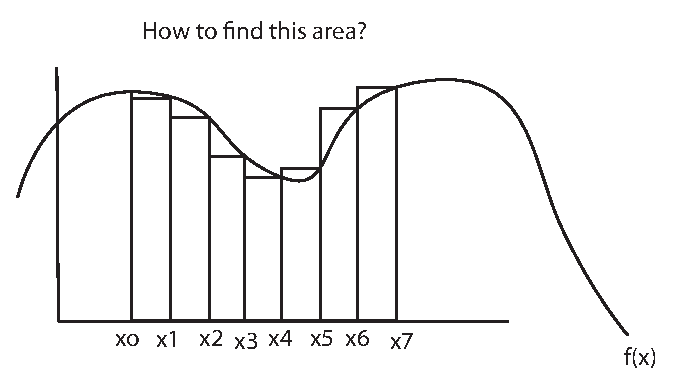
\epsfig{file=question2.eps, scale=.7}
  \end{center}
  \newslide
  
 \begin{center}
  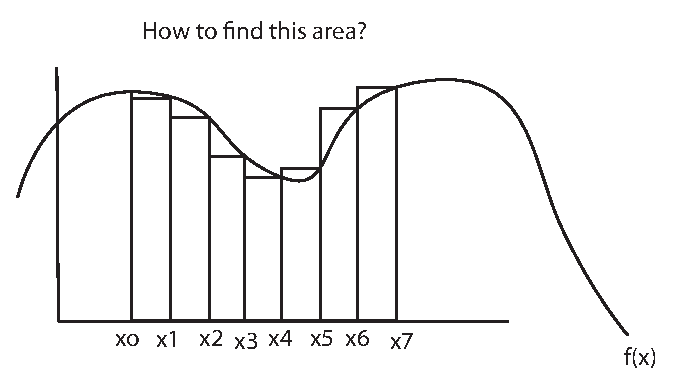
\epsfig{file=question2.eps, scale=.5}
  \end{center}
  
  $\sum_{i=1}^7 (x_i-x_{i-1})f(x_i)$  or letting $Dx_i=x_i-x_{i-1}$ this approximation is
$\sum_{i=1}^7 f(x_i) Dx_i$

\ \\Letting $\lim_{Dx_i}\rightarrow 0$ gives us the solution; it's written $$\int_a^b f(x) dx$$
  
  
  \newslide
  
  Areas below the $x-$axis are negative: $$\int_a^b f(x)=\hbox{Area(A)-Area(B)}$$
  
   \begin{center}
  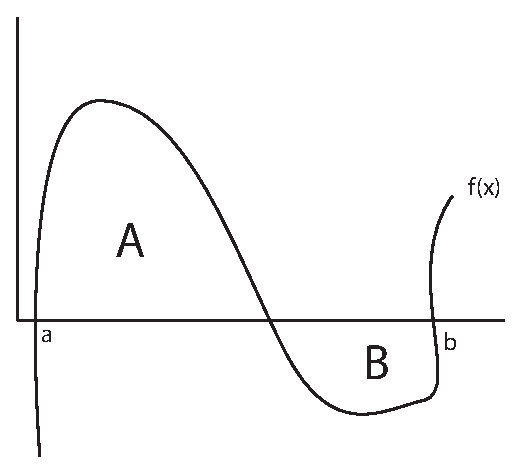
\epsfig{file=negative.eps, scale=.5}
  \end{center}
  
  
  \newslide
  
  A few properties of integrals
    \vspace{.3in}
  \begin{itemize}
  \item If $k$ is a constant then $\int_a^b k dx = k(b-a)$ \\(easy to see)
  \vspace{.3in}
  \item $\int_a^b x dx = {1\over 2}(b^2-a^2)$
  \vspace{.3in}
    \item $\int_a^b f(x) dx =\int_a^c f(x) dx + \int_c^b f(x) dx$ for $a\leq c\leq b$ \\(and for all $c$ in general)
  \end{itemize}
 

\newslide

 $$\int_a^b x dx = {1\over 2}(b^2-a^2)$$
 
    \begin{center}
  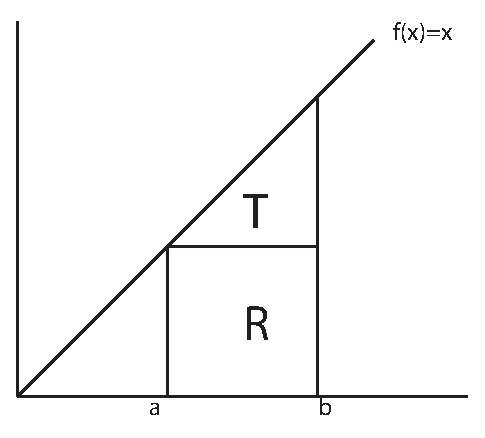
\epsfig{file=yx.eps, scale=.5}
  \end{center}
 
 This is $T+R$. $$R=(b-a)(a) \hbox{ and }T={1\over 2}(b-a)(b-a)$$
 $$R+T=ab-a^2+{1\over 2}b^2-ab+{1\over 2}a^2 = {1\over 2}(b^2-a^2)$$
 
 \newslide
 
The fundamental theorem of calculus
 
 \ \\Given a number $a$ and a continuous function $f(x)$ we can define another function $F$ such that $$F(t)=\int_a^t f(x) dx \hbox{ for all } t$$
 
 \ \\Then $F$ is differentiable and $F^\prime(t)=f(t)$ for all $t$
 
 \ \\If you integrate a function and then differentiate the result, you retrieve the function that you started with  $\Rightarrow$ ``integration is the reverse of differentiation"
 
 \newslide
     \begin{center}
  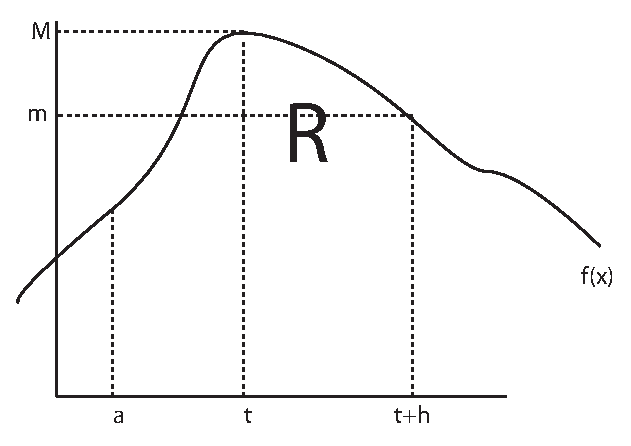
\epsfig{file=fundamental.eps, scale=.5}
  \end{center}
 
 Proof: Let $R=\int_t^{t+h}f(x) dx$ and let $F(t)=\int_a^t f(x) dx \hbox{ for all } t$.  Then $$R=\int_a^{t+h}f(x)dx-\int_a^{t}f(x)dx=F(t+h)-F(t)$$ We also have that $$ hm\leq F(t+h)-F(t)\leq hM, \hbox{ or }$$
$$m\leq {{F(t+h)-F(t)}\over{h}}\leq M$$ 
 
 \newslide
 
\begin{center}
  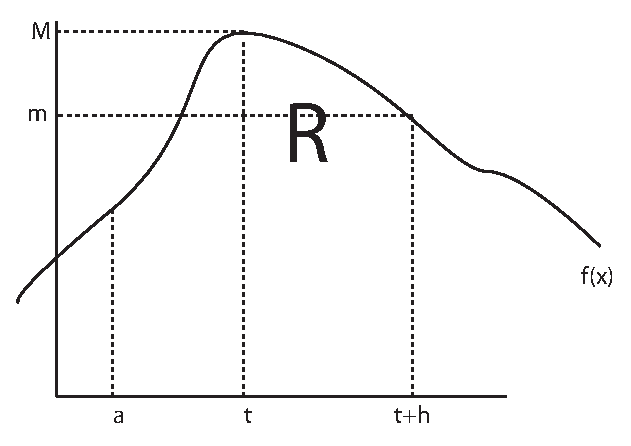
\epsfig{file=fundamental.eps, scale=.5}
  \end{center}

As $h\rightarrow 0$ we have $m\rightarrow f(t)=M$. Thus,

$$m\leq {{F(t+h)-F(t)}\over{h}}\leq M$$  implies that $$\lim_{h\rightarrow 0}{{F(t+h)-F(t)}\over{h}} =f(t)$$
or that $$F^\prime(t)=f(t) \hspace{.2in }\Box$$

%\newslide

%The fundamental theorem of calculus (again)

%\ \\Given a number $a$ and a continuous function $f(x)$ we can define another function $F$ such that $$F(t)=\int_a^t f(x) dx \hbox{ for all } t$$

% \ \\Then $F$ is differentiable and $F^\prime(t)=f(t)$ for all $t$

%\ \\You may be wondering: Why is $F(t)$ not also a function of $a$?

\newslide

Proposition: If $g$ has a continuous derivative, then $$\int_a^b g^\prime(x)=g(b)-g(a)$$ Proof: Let $$H(t)=g(t)-\int_a^t g^\prime(x) dx$$ Then $$H^\prime(t)=g^\prime(t)-g^\prime(t)=0 \hbox{ for all } t$$ Therefore $H$ is a constant, and $H(a)=H(b)$ for all $a, b$.  $$H(a)=g(a)-\int_a^a g^\prime(x) dx= g(a)$$ and since $H(a)=H(b)$, it must be that $H(b)=g(a)$ also. Therefore

$$g(a)-\int_a^a g^\prime(x) dx=g(b)-\int_a^b g^\prime(x) dx, \hbox{ or} $$ $$\int_a^b g^\prime(x)=g(b)-g(a) \hspace{.1in}\Box$$

\newslide
Takeaway point:

\ \\ To take an integral of $f(x)$ with bounds of integration $(a,b)$ you find the function that $f$ is the derivative of (call it $g(x)$) and then evaluate $g(b)-g(a)$.

\ \\We call $g$ the \textit{primitive} of $f$, so that $$g^\prime(x)=f(x) \hbox{ for all } x$$

\newslide

A few examples that we can actually solve

\ \\Example 1: $\int_2^3 x^2 dx$

\ \\Example 2: $\int_1^2 5-x^{-1} dx$

\ \\Example 3: $\int_{-1}^1 x dx$

\newslide
Indefinite integrals

\ \\If $g(x)$ is a primitive of $f(x)$ (so that $g^\prime(x)=f(x)$), then the set of all primitives of $f(x) $ is the set of all functions of the form $g(x)+C$, where $C$ is any constant.  $C$ is known as the \textit{constant of integration}

\ \\Let $f(x)=x+7$; we know that a primitive of $f(x)$ is $g(x)={1\over 2}x^2+7x$

\ \\It's also the case that $\tilde{g}(x)={1\over 2}x^2+7x+23$ is a primitive of $f$

\ \\Given a function $f$, the set of \textit{all} its primitives is the \textit{indefinite integral} of $f$, and is written $$\int f(x) dx$$

\newslide

Example: The indefinite integral  $\int 12x^2 dx=4x^3+C$, where $C$ is an arbitrary constant

\vspace{.2in}

\begin{itemize}
\item [Rule 1] $$\int x^\alpha dx={{1}\over{\alpha+1}}x^{\alpha+1}+C \hbox{ if }\alpha\not=-1$$

\item [Rule 2] $$\int {1\over x} dx=\ln x+C $$

\item [Rule 3] $$\int e^x dx =e^x +C$$

\end{itemize}

\newslide 

\begin{itemize}
\item [Rule 1'] $$\int (x-a)^\alpha dx={{1}\over{\alpha+1}}(x-a)^{\alpha+1}+C \hbox{ if }\alpha\not=-1$$

\item [Rule 2'] $$\int {1\over {(x-a)}} dx=\ln (x-a)+C \hbox{ if }x>a$$

\item [Rule 3'] $$\int e^{ax} dx ={{e^{ax}}\over{a}} +C$$

\end{itemize}


\newslide
Definite integrals

\ \\With definite integrals we do not need to worry about the constant of integration: We know that $$\int_a^b g^\prime(x) dx=g(b)-g(a)$$ If we used $g(x)+C$ as our primitive instead we'd get $$\int_a^b g^\prime(x) dx=(g(b) +C)-(g(a)+C)=g(b)-g(a)$$


\newslide

How you will most likely use integration: taking expected values

\vspace{.2in}

Suppose that there are 10 possible states of the world that each have a different probability of arising, and that each yield a different payoff

\begin{center}
\begin{tabular}{c||c|c|c|c|c|c|c|c|c|c|}
State & a&b &c&d&e&f&g&h&i&j\\
Probability & .05&.1 &.2&0&.1&.3&.05&0&.1&.1\\ \hline 
Payoff & x& 14& 3z&2&0&0&1&2x&3&40

\end{tabular}
\end{center}
\vspace{.2in}
What is my expected payoff?

\newslide



How you will most likely use integration: taking expected values

\vspace{.2in}

Suppose that there are 10 possible states of the world that each have a different probability of arising, and that each yield a different payoff

\begin{center}
\begin{tabular}{c||c|c|c|c|c|c|c|c|c|c|}
State & a&b &c&d&e&f&g&h&i&j\\
Probability & .05&.1 &.2&0&.1&.3&.05&0&.1&.1\\ \hline 
Payoff & x& 14& 3z&2&0&0&1&2x&3&40

\end{tabular}
\end{center}
\vspace{.2in}
What is my expected payoff?

\ \\(5.75+.05x+.6z)
\newslide

$f(x)$ is the probability density function (pdf) of a random variable $X$ if it satisfies the following: 

\begin{itemize}
\item For all $a\in \mathbb{R}$, $f(x)\geq 0$
\item $\int_{-\infty}^{\infty}f(x)dx =1$
\end{itemize}

\ \\The expected value of the random variable is $E[X]=\int_{-\infty}^{\infty}x f(x) dx$

\ \\The integral of a function of a random variable multiplied by the pdf gives the expected value of that function (like a weighted average)

\newslide

The uniform distribution over $[a, b]$ has pdf $f(x)={1\over{b-a}}$ for $x\in [a,b]$ and $f(x)=0$ otherwise

\ \\Check that $f(x)$ is really a pdf, so that $\int_{-\infty}^{\infty}f(x) dx =1$

\ \\Find the expected value of $X$ when $X$ is distributed  $U[0, 1]$

\ \\What is the expected value of $x^2$ when $X$ is distributed $U[0, 1]$?

\ \\What is the expected value of $x^2$ when $X$ is distributed $U[2, 10]$?


 \end{slide}
 
 \end{document}








